\documentclass[a4,useAMS,usenatbib,usegraphicx]{latex/mn2e} 
%\documentclass{latex/emulateapj} 
%External Packages and personalized macros
%=========================================================================
%		EXTERNAL PACKAGES
%=========================================================================
\usepackage{amsmath} 
\usepackage{amssymb} 
\usepackage[section]{placeins}
\usepackage {graphicx}
%\usepackage{graphics}
\usepackage[dvips]{epsfig}
\usepackage{epsfig}  
\usepackage{color}
\usepackage[normalem]{ulem}
\usepackage{hyperref}
\usepackage{caption}
%Non reposionated tables
\usepackage{float}
\restylefloat{table}

%=========================================================================
%		INTERNAL MACROS
%=========================================================================
\def\be{\begin{equation}}
\def\ee{\end{equation}}
\def\ba{\begin{eqnarray}}
\def\ea{\end{eqnarray}}

% To highlight comments 
\definecolor{red}{rgb}{1,0.0,0.0}
\newcommand{\red}{\color{red}}
\definecolor{darkgreen}{rgb}{0.0,0.5,0.0}
\newcommand{\SRK}[1]{\textcolor{darkgreen}{\bf SRK: \textit{#1}}}
\newcommand{\SRKED}[1]{\textcolor{darkgreen}{\bf #1}}

\newcommand{\LCDM}{$\Lambda$CDM~}
\newcommand{\beq}{\begin{eqnarray}}  
\newcommand{\eeq}{\end{eqnarray}}  
\newcommand{\zz}{$z\sim 3$} 
\newcommand{\apj}{ApJ}  
\newcommand{\apjs}{ApJS}  
\newcommand{\apjl}{ApJL}  
\newcommand{\aj}{AJ}  
\newcommand{\mnras}{MNRAS}  
\newcommand{\mnrassub}{MNRAS accepted}  
\newcommand{\aap}{A\&A}  
\newcommand{\aaps}{A\&AS}  
\newcommand{\araa}{ARA\&A}  
\newcommand{\nat}{Nature}  
\newcommand{\physrep}{PhR}
\newcommand{\pasp}{PASP}    
\newcommand{\pasj}{PASJ}    
\newcommand{\avg}[1]{\langle{#1}\rangle}  
\newcommand{\ly}{{\ifmmode{{\rm Ly}\alpha}\else{Ly$\alpha$}\fi}}
\newcommand{\hMpc}{{\ifmmode{h^{-1}{\rm Mpc}}\else{$h^{-1}$Mpc }\fi}}  
\newcommand{\hGpc}{{\ifmmode{h^{-1}{\rm Gpc}}\else{$h^{-1}$Gpc }\fi}}  
\newcommand{\hmpc}{{\ifmmode{h^{-1}{\rm Mpc}}\else{$h^{-1}$Mpc }\fi}}  
\newcommand{\hkpc}{{\ifmmode{h^{-1}{\rm kpc}}\else{$h^{-1}$kpc }\fi}}  
\newcommand{\hMsun}{{\ifmmode{h^{-1}{\rm {M_{\odot}}}}\else{$h^{-1}{\rm{M_{\odot}}}$}\fi}}  
\newcommand{\hmsun}{{\ifmmode{h^{-1}{\rm {M_{\odot}}}}\else{$h^{-1}{\rm{M_{\odot}}}$}\fi}}  
\newcommand{\Msun}{{\ifmmode{{\rm {M_{\odot}}}}\else{${\rm{M_{\odot}}}$}\fi}}  
\newcommand{\msun}{{\ifmmode{{\rm {M_{\odot}}}}\else{${\rm{M_{\odot}}}$}\fi}}  
\newcommand{\lya}{{Lyman$\alpha$~}}
\newcommand{\clara}{{\texttt{CLARA}}~}
\newcommand{\rand}{{\ifmmode{{\mathcal{R}}}\else{${\mathcal{R}}$ }\fi}}  
%SAMPLES
\newcommand{\GHBDM}{\texttt{GH}$_{\mbox{\tiny{BDM}}}$ }
\newcommand{\GHFOF}{\texttt{GH}$_{\mbox{\tiny{FOF}}}$ }
\newcommand{\IHBDM}{\texttt{IH}$_{\mbox{\tiny{BDM}}}$ }
\newcommand{\IHFOF}{\texttt{IH}$_{\mbox{\tiny{FOF}}}$ }
\newcommand{\PBDM}{\texttt{P}$_{\mbox{\tiny{BDM}}}$ }
\newcommand{\PFOF}{\texttt{P}$_{\mbox{\tiny{FOF}}}$ }
\newcommand{\IPBDM}{\texttt{IP}$_{\mbox{\tiny{BDM}}}$ }
\newcommand{\IPFOF}{\texttt{IP}$_{\mbox{\tiny{FOF}}}$ }
\newcommand{\RIPBDM}{\texttt{RIP}$_{\mbox{\tiny{BDM}}}$ }
\newcommand{\RIPFOF}{\texttt{RIP}$_{\mbox{\tiny{FOF}}}$ }


%MY COMMANDS #############################################################
\newcommand{\sub}[1]{\mbox{\scriptsize{#1}}}
\newcommand{\dtot}[2]{ \frac{ d #1 }{d #2} }
\newcommand{\dpar}[2]{ \frac{ \partial #1 }{\partial #2} }
\newcommand{\pr}[1]{ \left( #1 \right) }
\newcommand{\corc}[1]{ \left[ #1 \right] }
\newcommand{\lla}[1]{ \left\{ #1 \right\} }
\newcommand{\bds}[1]{\boldsymbol{ #1 }}
\newcommand{\oiint}{\displaystyle\bigcirc\!\!\!\!\!\!\!\!\int\!\!\!\!\!\int}
\newcommand{\mathsize}[2]{\mbox{\fontsize{#1}{#1}\selectfont $#2$}}
\newcommand{\eq}[2]{\begin{equation} \label{eq:#1} #2 \end{equation}}
\newcommand{\lth}{$\lambda_{th}$ }
%#########################################################################

\begin{document}

%=========================================================================
%		FRONT MATTER
%=========================================================================
\title{Fractional anisotropy as a tracer of cosmic voids}
\author[S. Bustamante and J.E. Forero-Romero]{
\parbox[t]{\textwidth}{\raggedright 
  Sebastian Bustamante \thanks{sebastian.bustamante@udea.edu.co}$^{1}$,
  Jaime E. Forero-Romero$^{2}$ 
}
\vspace*{6pt}\\
$^1$Instituto de F\'{\i}sica - FCEN, Universidad de Antioquia, Calle
67 No. 53-108, Medell\'{\i}n, Colombia\\ 
$^2$Departamento de F\'{i}sica, Universidad de los Andes, Cra. 1
No. 18A-10, Edificio Ip, Bogot\'a, Colombia
}

\maketitle

\begin{abstract}
Finding and characterizing voids in the large scale structure of the
universe is an important task in cosmological studies. 
In this paper we present a novel approach to find voids in
cosmological simulations.  
It is based on algorithms that use the tidal and the
velocity shear tensors to define the cosmic web.
Voids are identified using the fractional anisotropy (FA) computed
from the eigenvalues of each web scheme. We define the void boundaries
using a watershed transform based on the local minima of the FA; the
boundaries are regions where the FA is maximized, corresponding to
walls and filaments.  This void definition does not have any free
parameter and does not make any assumption on the shape or structure
of the voids.  We test the method on the Bolshoi simulation and report
on the density and velocity profiles for the voids found using this
new scheme.
\end{abstract}

\begin{keywords}
Cosmology: theory - large-scale structure of Universe -
Methods: data analysis - numerical - N-body simulations
\end{keywords}


%=========================================================================
%		PAPER CONTENT
%=========================================================================

%*************************************************************************
\section{Introduction}
\label{sec:introduction}
%*************************************************************************


Since voids where discovered in the first compiled galaxy surveys 
\citep{Chincarini75, Gregory78, Einasto80M, Einasto80N, Kirshner81, 
Kirshner87}, they have been identified, along with the filamentary and 
hierarchically clustered nature of the Cosmic Web, as one of the most 
striking features of the Megaparsec Universe \citep{Bond96}. Nevertheless,
due to the large volume extension of void regions ($\sim 5-10\ \mbox{Mpc} 
h^{-1}$), statistically meaningful catalogues of voids \citep{Pan10, 
Sutter12b, Nadathur14} only have become available after modern large 
galaxy surveys like the two-degree field Galaxy Redshift Survey \citep{
Colless01, Colless03} and the Sloan Digital Sky Survey \citep{York00,
Abazajian03}, thereby triggering a plethora of more refined observational 
and statistical studies of voids throughout the last decade \citep{Hoyle04,
Croton04, Rojas05, Ceccarelli06, Patiri06a, Tikhonov06, Patiri06b, 
Tikhonov07, BendaBeckmann08, Foster09, Ceccarelli13, Sutter14a}


On the theoretical side, early descriptions of the evolution of the 
large-scale Universe, based on gravitational instabilities in primordial 
stages and leaded by the seminal work of \citet{Zeldovich70}, are 
consistent with the Cosmic Web picture, where planar pancake-like regions 
of matter enclose enormous underdense voids and are bordered, in turn, by 
thin filaments and high-density clumpy knots \citep{Bond96}. First 
theoretical models for describing formation, dynamics and properties of 
voids \citep{Hoffman82, Icke84, Bertschinger85, Blumenthal92} were 
dramatically complemented and extended by first numerical studies based 
on simulations \citep{Martel90, Regos91, Weygaert93, Dubinski93}. This 
tendency of using numerical data from N-body simulations, fuelled by last 
generation computing systems and ever more efficient numerical algorithms, 
has become increasingly common in the last years as a powerful analysis 
toolkit of cosmic voids (for an extensive compilation of previous 
numerical works, see \citet{Colberg08}).


At present, studying voids may be considered as a threefold enterprise
\citep{Platen07}: first, they are a key ingredient of the Cosmic Web as 
they dominate almost the entire volume distribution at large-scales and 
additionally, they compensate overdense structures in the total budget of 
matter. This implies that a full understanding of their evolution and 
properties is essential for fathoming the high complexity of the Cosmic 
Web. Second, they provide a valuable resource for inferring and probing 
cosmological parameters as their structure and dynamics are highly 
determined by these values. Third, they constitute an unique and still 
largely pristine environment in which can be tested galaxy evolution.


Although a visual recognition of voids in galaxy surveys and simulations
is possible in most cases, a formal systematic identification is necessary 
for statistically meaningful studies. However, a basic yet essential issue 
remains regarding the definition itself of what a void is. There is not a 
general consensus about an unambiguous definition of cosmic voids and 
therefore, there can be found many different void finding techniques 
throughout the literature (for a detailed comparison of different schemes, 
see the Void Finder Comparison Project \citet{Colberg08}). In spite of the 
diversity of existing schemes, they can be roughly classified into two 
main types: first, geometric schemes based on point spatial or redshift 
distribution of galaxies in surveys or catalogues of dark matter halos in 
simulations \citep{Kauffmann91, Muller00, Gottlober03, Hoyle04, Brunino07, 
Foster09, Micheletti14, Sutter14}, and second, schemes based on the smooth 
and continuous matter density field either from simulations or from 
reconstruction procedures on surveys \citep{Plionis02, Colberg05, 
Shandarin06, Platen07, Neyrinck08, Neyrinck13, Ricciardelli2013}.


Here we introduce a new tracer of the structure of cosmic voids built from 
two tensorial web schemes, i.e. the Tweb, based on the Hessian of the 
gravitational potential or tidal tensor \citep{Hahn07, Forero09}, and the 
Vweb, based on the velocity shear tensor \citep{Hoffman12}. These web 
schemes classify the Cosmic Web into four different types of environment
depending on the counting of the number of eigenvalues below an 
user-defined threshold ($\lambda_{th}$), namely voids (3 eigenvalues below
$\lambda_{th}$), sheets (2), filaments (1) and knots or clusters (0).
The tidal and the shear tensors have proven to be more fundamental than 
the density field as they also trace the collapsing or expanding nature of 
the matter field, which ultimately is what defines the underlying dynamics 
of the Cosmic Web. Furthermore, the density field is degenerated regarding 
the defined types of environment \citep{Hahn07}, which implies that is not 
possible to assign a priori a range of density values to each of them. 
This yields that the usually adopted definition of voids as simply 
underdense regions in the large-scale matter distribution, is not precise 
enough as it excludes a proper description of the internal structure of 
voids.


Following the recent trend of using digital image-processing techniques 
developed in other disciplines (e.g. medical sciences and computer imaging) 
for analysing the structure of the Cosmic Web, we propose here, much in 
the same way as \citet{Libeskind13}, the fractional anisotropy (FA) as a 
tracer of the internal structure and the outline of cosmic voids. The FA 
was initially introduced by \citet{Basser95} for quantifying the 
anisotropy degree of the diffusivity of water molecules through cerebral
tissue in nuclear magnetic resonance imaging. In this context we use the 
same quantity for determining the anisotropy degree of the local 
environment from either the orbital dynamics as set by the eigenvalues of
the tidal tensor (Tweb), or the dynamics of the velocity field as set by 
the eigenvalues of the shear tensor (Vweb). In both cases, the FA is not
determined directly from the density field, it hence is suitable for 
describing both, the structure of high non-linear regions (e.g. filaments,
knots and very dense walls) as well as the fainter substructure exhibited 
by quasi-linear regions like voids.


Once established the FA as the tracer field of cosmic voids, we proceed to
identify individual voids as basins of local minima. For this purpose we
implement a technique developed by \citet{Beucher79} and \citet{Beucher93} 
and widely used in the field of image analysis and mathematical morphology, 
i.e. the \textit{watershed transform algorithm}. This technique has been 
already implemented on void finding schemes by \citet{Platen07} and 
\citet{Neyrinck08} with very interesting results, where individual voids 
are identified as catching basins of local minima of the density field. 
The appeal of this algorithm consists in that is parameter-free and does 
not require any assumption on the shape and morphology of voids. 
Although we use a \textit{cloud-in-cell} (\texttt{CIC}) algorithm on a 
Cartesian mesh for estimating the density and tensor fields, instead of 
the more sophisticated \textit{Delaunay tessellation for field estimator} 
(\texttt{DTFE}) technique \citep{Schaap00}, our implementation of the 
watershed transform should not be significantly affected as we are 
interested in quasi-linear regions where the \texttt{CIC} gives similar 
estimations.


This paper is organized as follows. In section 2 we describe the used
simulation for testing our void finding algorithm, i.e. the Bolshoi
simulation. Alternatively to the web schemes Tweb and Vweb, we propose 
a heuristic web classifier based on three thresholds of the density field. 
This is used in order to illustrate the differences of our scheme with a
density-based classifier. A detailed description of these methods is 
presented in section 3. In section 4 we describe how the FA can be used 
for tracing the structure of voids. Once obtained meaningful catalogues 
of voids for each scheme, we proceed to compare some typical and general 
interest properties of voids such as volume functions, distributions of 
size and density and velocity profiles. This is done in section 5. Finally 
in section 6 we analyse and evaluate our findings.



%*************************************************************************
\section{The Simulation}
\label{sec:the_simulation}
%*************************************************************************


We use here an unconstrained cosmological simulation (the Bolshoi 
simulation) to identify the possible large scale environment and the 
distribution of cosmic voids at $z=0$. The Bolshoi simulation follows the 
non-linear evolution of a dark matter density field on a cubic volume of 
size $250$\hMpc sampled with $2048^3$ particles. The cosmological 
parameters in the simulation are $\Omega_{\rm m}=0.27$, $\Omega_{\Lambda}
=0.73$, $h=0.70$, $n=0.95$ and $\sigma_{8}=0.82$ for the matter density, 
cosmological constant, dimensionless Hubble parameter, spectral index of 
primordial density perturbations and normalization for the power spectrum
respectively, consistent with the seventh year of data of the Wilkinson 
Microwave Anisotropy Probe (WMAP) \citep{Jarosik11}. For more detailed 
technical information about the simulation, see \citet{Klypin11}.


For estimating the density and velocity fields we use a 
\textit{cloud-in-cell} (\texttt{CIC}) algorithm onto a grid of $256^3$ 
cells, corresponding to a resolution of $0.98$\hMpc per cell side. Then, 
through finite-differences and FFT methods the tidal and shear tensors 
are computed. Finally, the eigenvalues and eigenvectors of the tensor are
obtained for each cell of the grid. Neglecting substructures presented 
below Megaparsec scales and taking into account our focus in voids, which
are a prominent characteristic of the Megaparsec Universe, we apply a 
Gaussian softening of one cell to all fields.



%*************************************************************************
\section{Algorithms to quantify the Cosmic Web}
\label{sec:algorithms_cosmic_web}
%*************************************************************************


%-------------------------------------------------------------------------
\subsection{The tidal web (Tweb)}
\label{subsec:Tweb}
%-------------------------------------------------------------------------


This scheme was initially proposed by \citet{Hahn07} as a novel 
alternative for classifying the Cosmic Web based on the tidal tensor, 
that is somehow more fundamental than the density field as it also allows 
to quantify the orbital dynamics of the matter field. This approach 
consists of a second-order expansion of the equations of motion around 
local minima of the gravitational potential and then extended to any 
position. The second-order term corresponds to the tidal tensor, which is
defined as the Hessian matrix of the normalized gravitational potential


%.........................................................................
%Tidal Tensor
\eq{V_web}
{	T_{\alpha\beta} = \frac{\partial^2\phi}{\partial x_{\alpha}\partial x_{\beta}}	}
%.........................................................................
where the physical gravitational potential has been rescaled by a factor 
$4\pi G\bar{\rho}$ in such a way that $\phi$ satisfies the following 
equation


%.........................................................................
%Poisson
\eq{Poisson}
{	\nabla^2\phi = \delta,	}
%.........................................................................
with $\bar{\rho}$ the average density in the Universe, $G$ the 
gravitational constant and $\delta$ the dimensionless matter overdensity.


Since the tidal tensor can be represented in any cell by a real and 
symmetric $3\times 3$ matrix, it is ensured the possibility to diagonalize 
it and obtain three real eigenvalues $\lambda_{1}\geq\lambda_{2}\geq
\lambda_3$. This set of eigenvalues can be used as indicators of the local 
orbital stability in each proper direction, which in turn can be 
translated into a classification scheme of the Cosmic Web. A counting of 
the number of positive (stable) or negative (unstable) eigenvalues allows 
to catalogue a single cell into one of the next four types of environment: 
voids (3 negatives eigenvalues), sheets (2), filaments (1) and knots (0). 
A significant improvement to this scheme was introduced by \citet{Forero09}
by means of a relaxation of the stability criterion. The relative strength 
of each eigenvalue is no longer defined by the sign, but instead by a
threshold value $\lambda_{th}$ that can be tuned in such a way that the
visual impression of the web-like matter distribution is reproduced.



%-------------------------------------------------------------------------
\subsection{The velocity web (Vweb)}
\label{subsec:Vweb}
%-------------------------------------------------------------------------


We also use a kinematical scheme to define the Cosmic Web environment in 
the simulation. The scheme has been thoroughly described in 
\citet{Hoffman12} and applied to study the shape and spin alignment in the
Bolshoi simulation in \citet{Libeskind13}. We refer the reader to these 
papers to find a detailed description of the algorithm, its limitations 
and capabilities. The Vweb scheme for environment finding is based on the
local velocity shear tensor calculated from the smoothed dark matter 
velocity field in the simulation. The central quantity is given by the 
following dimensionless expression


%.........................................................................
%V-Web Definition
\eq{V_web}
{	\Sigma_{\alpha\beta} = -\frac{1}{2H_0}\pr{\frac{\partial v_{\alpha}}
{\partial x_{\beta}}+\frac{\partial v_{\beta}}{\partial x_{\alpha}}}	}
%.........................................................................
where $v_{\alpha}$ and $x_{\alpha}$ represent the $\alpha$ component of 
the comoving velocity and position, respectively. Like the tidal tensor, 
$\Sigma_{\alpha\beta}$ can be represented by a $3\times 3$ symmetric 
matrix with real values, hence diagonalizing it is obtained three real 
eigenvalues $\lambda_{1}\geq\lambda_{2}\geq\lambda_3$ whose sum (the 
trace of $\Sigma_{\alpha\beta}$) is proportional to the divergence of the 
local velocity field smoothed on the physical scale ${\mathcal R}$. 


In the same way, the relative strength of the three eigenvalues with 
respect to a threshold value $\lambda_{th}$ allows for the local 
classification of the matter distribution into the previous four web types. 
For the threshold choosing in both schemes, the Tweb and the Vweb, it is
usual to fine-tuning the value in such a way that the visual appearance of
the Cosmic Web as seen in simulations and galaxy surveys is reproduced. 
However, we do not take this approach here, instead we propose a novel 
approach for the threshold choosing based on the maximization of the 
fractional anisotropy field occurring in filaments and very dense walls.


%-------------------------------------------------------------------------
\subsection{The density-based web finder}
\label{subsec:Vweb}
%-------------------------------------------------------------------------


Although the density field is a key quantity for understanding the 
large-scale Universe, the filamentary structure of the Cosmic Web is 
poorly traced by it (see e.g. Fig. \ref{fig:FA_field}). In order to 
compare our new proposal based on the the fractional anisotropy as a 
tracer field of voids, we define a very basic approach for environmental 
finding based on three thresholds of the density field. 


%.........................................................................
%Table with volume filling fraction
\begin{table}[h]
\begin{flushleft}
\begin{center}
  \begin{tabular}{c  c  c  c c} \hline\hline
	\textbf{Volume}  &				&\textbf{Scheme}& \\
	\textbf{Filling} &				&				&					  &  \textbf{Threshold} \\ 
	\textbf{Fraction}&\textbf{Tweb}&\textbf{Vweb}	&	\textbf{Density}  &  $\bf{\delta_{th}}$  \\ \hline
	Voids			 &	$54.88\%$	&	$47.06\%$	&	$50.97\%$	 	  &	$ -0.57$			\\ 
	Sheets		     &	$33.21\%$	&	$39.54\%$	&	$36.38\%$ 	      &	$0.60$				\\
	Filaments		 &	$11.16\%$	&	$12.18\%$	&	$11.67\%$ 		  &	$8.82$				\\
	Knots			 &	$0.75\%$	&	$1.22\%$	&	$0.98\%$  		  &	--		\\ \hline\hline
  \end{tabular}  
  \captionof{table}{\small VFF for each type of environment and for each
  web scheme. VFF for the density-based scheme are defined as the 
  arithmetic mean of the Tweb and the Vweb. The last column corresponds 
  to the threshold values in the density field in order to obtain the 
  required VFF. Note there is not any value associated to knots as there 
  is not a higher order environment.}
  
  \label{tab:VFF}
\end{center}
\end{flushleft}
\end{table}
%.........................................................................


In next section we shall describe an alternative approximation to select 
the threshold value $\lambda_{th}$. One of the main results is the similar 
volume filling fraction (VFF) for each environment in both web schemes 
(see Fig. \ref{fig:VFF}). Using this result, we propose here a heuristic 
classification of the Cosmic Web based on three density thresholds 
assigned to each boundary (i.e. void-sheet, sheet-filament and 
filament-knot)\footnote{The progressive sequence void-sheet-filament-knot 
along any path through the Cosmic Web should be always satisfied as each 
used field is smoothed.} such that the corresponding VFF values are 
similar to the values obtained for the Tweb and the Vweb, specifically 
they are defined to be the arithmetic mean of both schemes.


%*************************************************************************
\section{Finding voids}
\label{sec:bulk_voids}
%*************************************************************************


%-------------------------------------------------------------------------
\subsection{Fractional anisotropy as tracer of voids}
\label{subsec:FA_voids}
%-------------------------------------------------------------------------


The fractional anisotropy (FA), as developed by \citet{Basser95}, was 
conceived to quantify the anisotropy degree of a diffusion process, e.g. 
the diffusivity of water molecules through cerebral issue in nuclear
magnetic resonance imaging. Here we propose the FA, much in the same 
way as \citet{Libeskind13}, as a tracer of cosmic voids.


%.........................................................................
%Fractional anisotropy
\eq{fractional_anisotropy}
{ FA = \frac{1}{\sqrt{3}}\sqrt{ \frac{ (\lambda_1 - \lambda_3)^2 + 
(\lambda_2 - \lambda_3)^2 + (\lambda_1 - \lambda_2)^2}{ \lambda_1^2 + 
\lambda_2^2 + \lambda_3^2} } }
%.........................................................................
where the eigenvalues are taken from either the Tweb or the Vweb 
(FA-Tweb and FA-Vweb respectively). Such as it is defined, $FA=0$ 
corresponds with a isotropic dynamic and $FA=1$ with a highly anisotropic 
distribution.


In left panels of Fig. \ref{fig:FA_field} we calculate the FA for both 
web schemes and the logarithmic density field over a slide of the 
simulation. Some important points can be concluded of this figure.


%.........................................................................
\begin{itemize}
\item Voids display a highly isotropic expanding dynamic at their centres, 
becoming gradually more anisotropic at outer regions.
\item Knots feature with very isotropic collapses. For the Tweb, the FA 
exhibits very narrow distribution around knots whereas for the Vweb, these
distributions are more spread out, thereby indicating strong differences 
between the density and the velocity fields in highly non-linear regions.
\item The filamentary structure of the Cosmic Web is very good traced by
high FA values (black regions), thus indicating very anisotropic dynamics 
for sheets and filaments.
\item The density field poorly traces the Cosmic Web. This is a somehow 
expected result due to the semi-infinite range of the density field, what 
makes more difficult to trace structures.
\end{itemize}
%.........................................................................


Some of these results are consistent with those of \citet{Libeskind13}.
Finally, from Fig. \ref{fig:FA_field} we conclude that the FA, unlike the
density field, displays a non-monotonic behaviour, where low values are 
characteristic of central regions of voids, reaching high values in sheets
and filaments and becoming low again in knots. 


For both web schemes, voids are regions where $\lambda_3\leq\lambda_2\leq
\lambda_1\leq\lambda_{th}$. This implies that the outlines of voids
are completely fixed by the relative strength of the $\lambda_1$ 
eigenvalue with respect to the threshold value. Therefore, as we 
increase/decrease the threshold value $\lambda_{th}$, voids expand/diminish
progressively through contours of $\lambda_1$. In Fig. 
\ref{fig:L1_correlations} we calculate the distribution of the FA as well
as of the density field with respect to $\lambda_1$ for both web schemes 
over all cells of the simulation.


From Fig. \ref{fig:L1_correlations} we conclude that the FA is a good
tracer of voids as is perfectly correlated with low values of $\lambda_1$. 
Then, it reaches a maximum value, namely sheets and filaments, for finally
reaching knots, which feature low FA values. This behaviour can be thought 
as a sort of one-dimensional tomography of the Cosmic Web. This 
characteristic allows us to propose an optimal threshold value for both 
web schemes where the FA is maximized. Specifically we propose a value of 
$FA=0.95$, corresponding with a threshold $\lambda_{opt}^T = 0.265$ for
the Tweb and $\lambda_{opt}^V = 0.175$ for the Vweb.  For a threshold 
above these values, voids would span over very anisotropic regions, which 
should correspond to sheets and filaments. A threshold below would imply 
very low volume filling fractions of voids and dominant sheets. Finally 
from the same figure, the density field do not correlate well with 
$\lambda_1$ (as calculated for both web schemes). Moreover, due to its 
monotonic increase, an estimate of a optimal threshold is not as clear as 
for the FA.


Once set the optimal thresholds for the web schemes, we proceed in Fig. 
\ref{fig:FAShapeness} to sample the FA along with the prolatenes for a 
random sample of cells classified into the four environments. Then, we 
associate a spheroidal geometry with different ranges of these properties
in order to illustrate the underlying local dynamics of the sampled cells.


From this figure we conclude that sheets displays, as expected, very 
anisotropic distributions, namely above $FA=0.95$. They are also biased 
towards oblate geometries, however there are some elongated sheets as 
well. Filaments are not as anisotropic as sheets, ranging from middle up 
to high FA values. They exhibit prolate geometries, but a considerable 
amount of them are biased towards slightly more oblate values. Voids and 
knots are the only environments featuring with low FA values, thus 
indicating very isotropic expanding/collapsing dynamics at their centres. 
However, voids span over a very wide range of FA and geometries, whereas 
knots only span over low to middle FA values and display a biased oblate 
geometry.


%-------------------------------------------------------------------------
\subsection{Identifying void regions through web schemes}
\label{subsec:identification}
%-------------------------------------------------------------------------




%*************************************************************************
\section{Properties of voids}
\label{sec:properties}
%*************************************************************************


Once defined our method to classify bulk voids based upon web 
classification schemes of the cosmic web, we proceed to analyse some 
physical properties in order to compare their consistency with the 
geometry of voids as quantified by our method and by density-based schemes.
Next, through the reduced inertia tensor we quantify the shape distribution 
of voids. Finally, we compute numerical radial profiles of density and 
peculiar velocity of bulk voids.


%-------------------------------------------------------------------------
\subsection{Statistics of halos in voids}
\label{subsec:shape_voids}
%-------------------------------------------------------------------------


One of the main challenges in observational void finding is the discrete 
nature of galaxy surveys

 we calculate contours of discrete fields like the median mass and 
the local number of local dark matter halos and

, like the inertia values,
the density and peculiar velocities profiles as calculated over the grid 
and profiles of number of halos.


%-------------------------------------------------------------------------
\subsection{Density profile of voids}
\label{subsec:density_voids}
%-------------------------------------------------------------------------


Describing the density profiles of voids is quite important in order to 
compare and match simulation with observational surveys, allowing possible
constrains for different cosmology models \SRKED{[Hamaous, et.al 2014]}. 
Here, and taking into account the previous results, we rather use an 
ellipsoidal approximation to describe and fit the shape of bulk voids, so 
we use the next ellipsoidal radial coordinate to describe density profiles.


%.........................................................................
%Ellipsoidal radial coordinate
\eq{radial_coordinate}
{
r^2 = \frac{x^2}{\tau_1^2} + \frac{y^2}{\tau_2^2} + \frac{z^2}{\tau_3^2},
\ \ \ \ 0\leq r \leq 1
}
%.........................................................................
where we take the principal moments of inertia $\{\tau_i \}$ as the 
lengths of the principal axes of the ellipsoid and each one of the 
cartesian coordinates as measured in the rotated frame of each void.


We use the same analytic density profile that \SRKED{[Hamaous, et.al 2014]} 
to fit the numerical density profiles of our voids.


%.........................................................................
%Density profile
\eq{density_profile}
{
\delta_v(r) = \delta_c\frac{1-(r/r_s)^\alpha}{1+(r/r_v)^\beta}
}
%.........................................................................



%*************************************************************************
\section{Conclusions}
\label{sec:conclusions}
%*************************************************************************


%*************************************************************************
\section*{Acknowledgments}  
%*************************************************************************


\bibliographystyle{latex/mn2e}
\bibliography{references}


%.........................................................................
%FIGURE 1: Volume Filling Fractions for environs
\begin{flushleft}
\begin{figure*}
\centering
  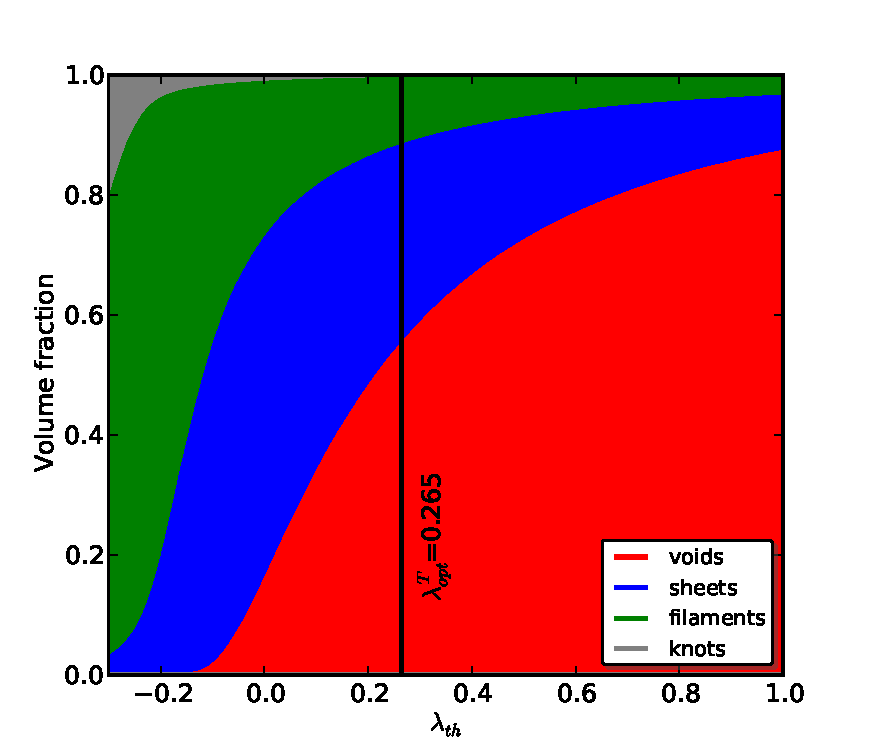
\includegraphics[trim = 2mm 2mm 5mm 6mm, clip, keepaspectratio=true,
  width=0.3\textheight]{./figures/cosmicweb_volume_Tweb.pdf}
  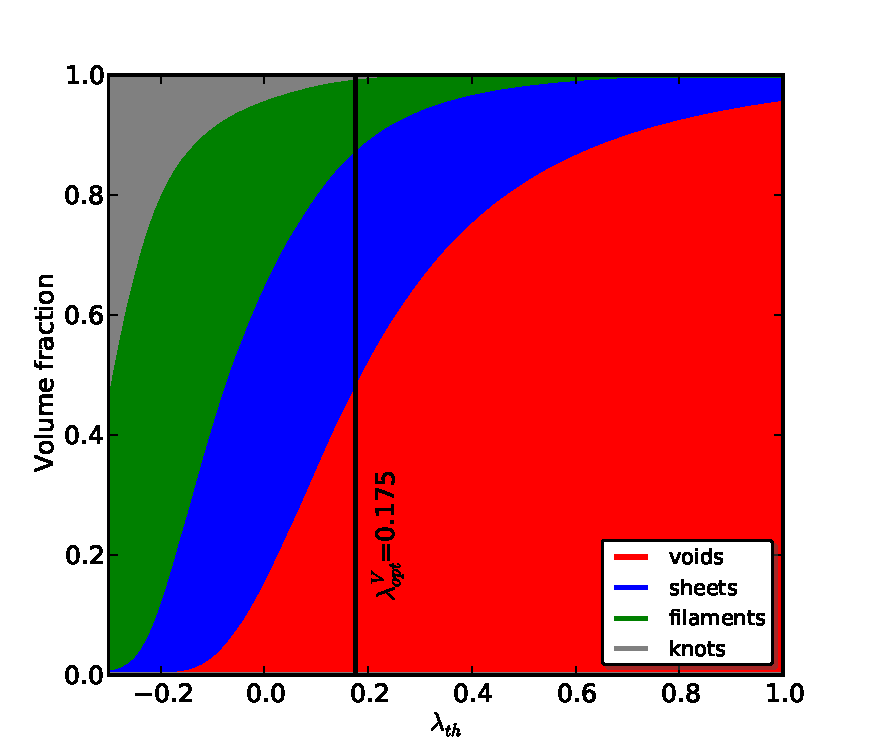
\includegraphics[trim = 2mm 2mm 5mm 6mm, clip, keepaspectratio=true,
  width=0.3\textheight]{./figures/cosmicweb_volume_Vweb.pdf}  
  
  \captionof{figure}{\small Volume Filling Fraction for each type of 
  environment with respect to the chosen threshold $\lambda_{th}$ for both
  web schemes (Tweb, left panel. Vweb, right panel). For each case, the 
  threshold value is chosen such that the fractional anisotropy along the 
  void-sheet boundaries has a median value of $FA=0.95$.}

  \label{fig:VFF}
  \vspace{0.1 cm}

\end{figure*}
\end{flushleft}
%.........................................................................


%.........................................................................
%FIGURE 2: Distributions of FA and density regarding the Lambda_1 eigenvalue
\begin{flushleft}
\begin{figure*}
\centering

  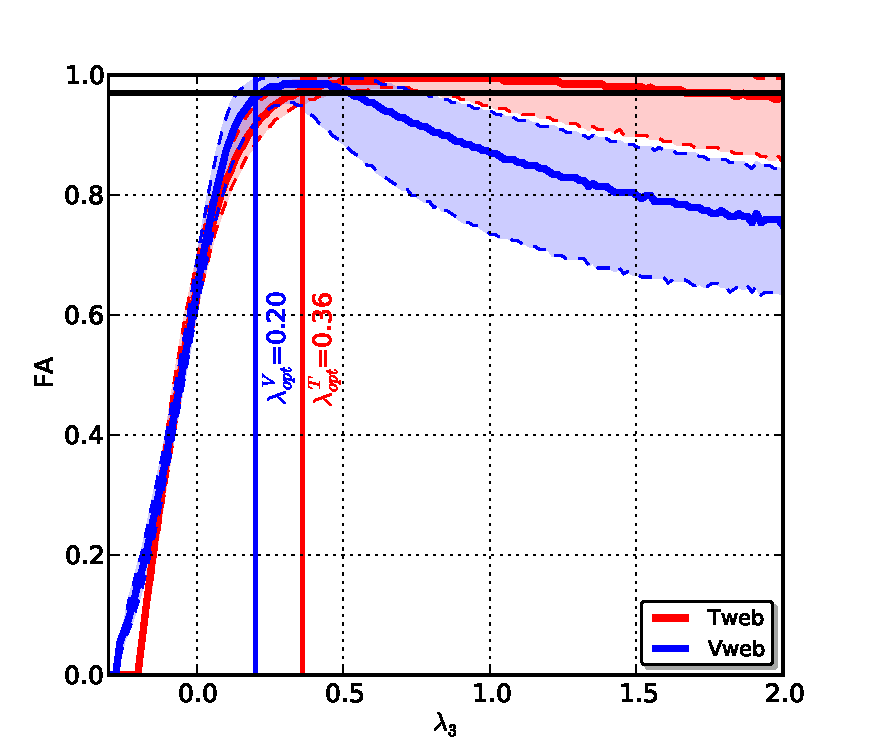
\includegraphics[trim = 2mm 2mm 5mm 10mm, clip, keepaspectratio=true,
  width=0.3\textheight]{./figures/FA_L1.pdf}
  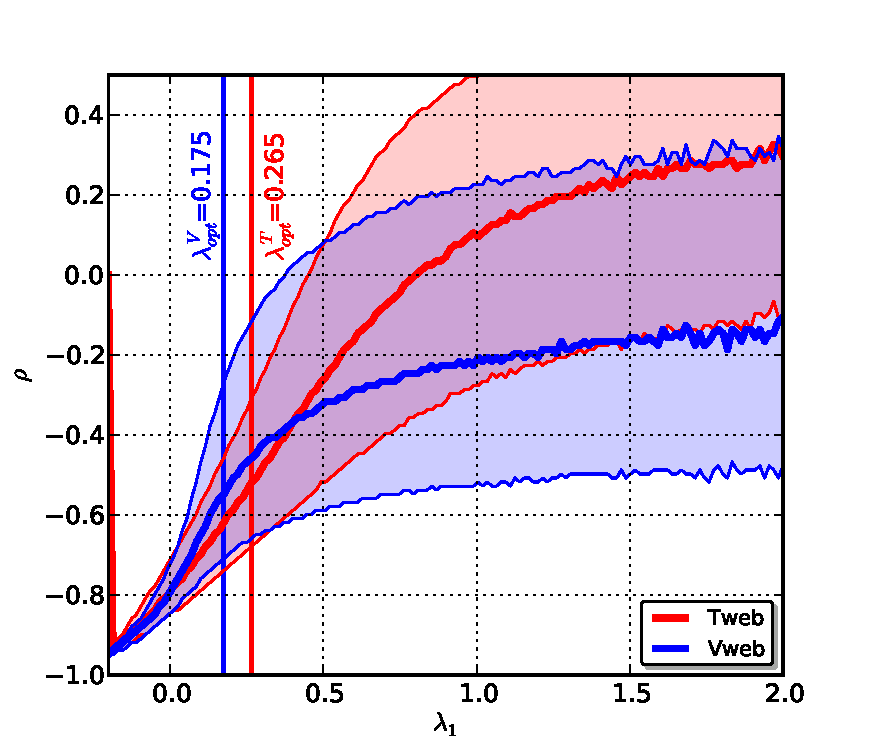
\includegraphics[trim = 2mm 2mm 5mm 10mm, clip, keepaspectratio=true,
  width=0.3\textheight]{./figures/delta_L1.pdf}  
  
  \captionof{figure}{\small Distributions of the fractional anisotropy 
  (left panel) and the density field (right panel) with respect to the 
  eigenvalue $\lambda_1$ for each web scheme (Tweb, red lines. Vweb, 
  blue lines) as calculated over all cells of the grid. Thick central 
  lines correspond with the median and filled regions with the $50\%$ of
  the distribution.}

  \label{fig:L1_correlations}
  \vspace{0.1 cm}

\end{figure*}
\end{flushleft}
%.........................................................................


%.........................................................................
%FIGURE 3: FA of some regions and shape illustration
\begin{flushleft}
\begin{figure*}
\centering

  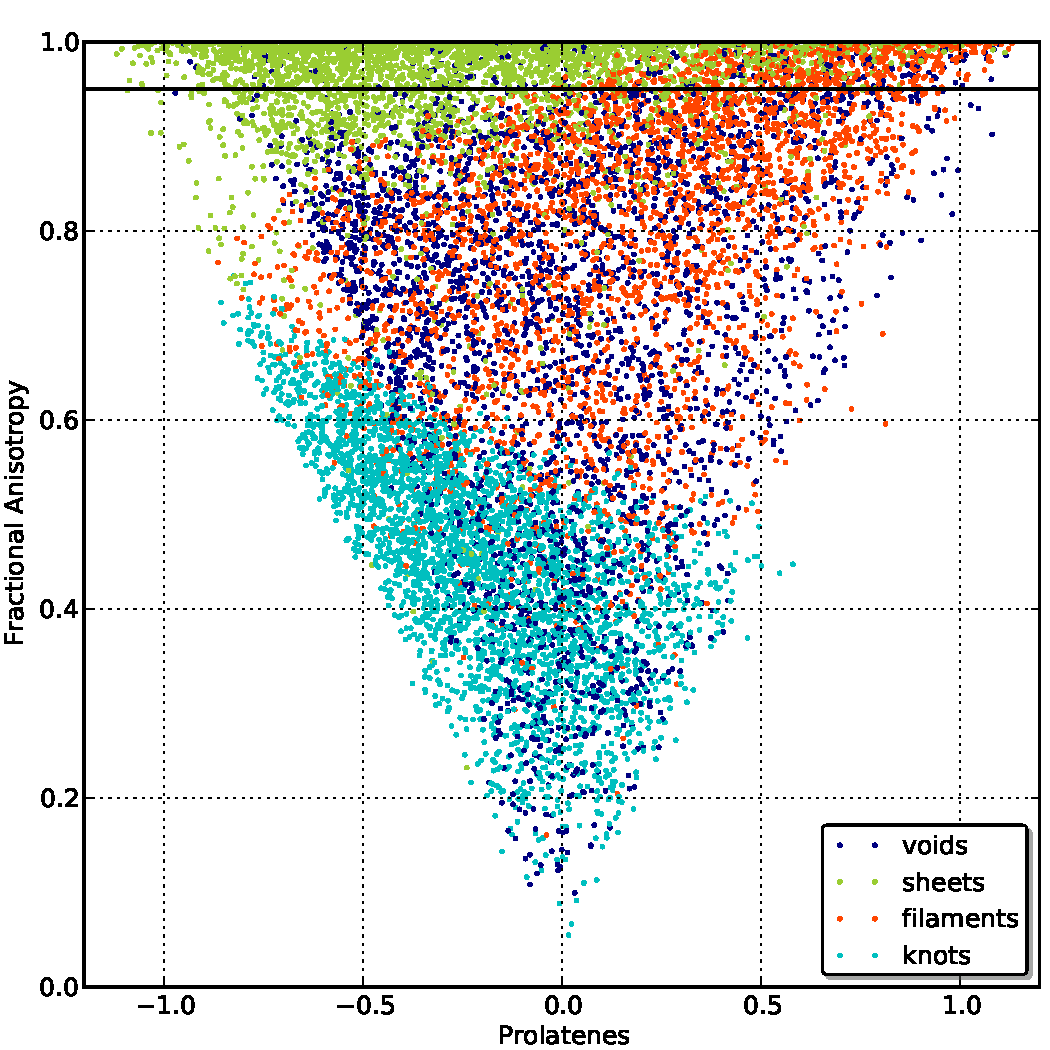
\includegraphics[trim = 0mm 1mm 0mm 1mm, clip, keepaspectratio=true,
  width=0.3\textheight]{./figures/FA_Prolatenes_Vweb.pdf}
  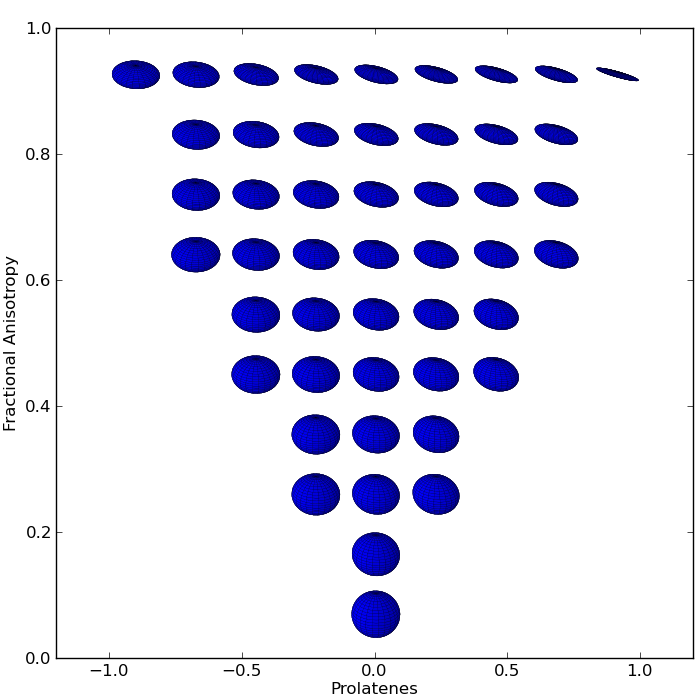
\includegraphics[trim = 0mm 1mm 0mm 1mm, clip, keepaspectratio=true,
  width=0.3\textheight]{./figures/FA_Prolatenes.png}  
  
  \captionof{figure}{\small }

  \label{fig:FAShapeness}
  \vspace{0.1 cm}

\end{figure*}
\end{flushleft}
%.........................................................................


%.........................................................................
%FIGURE 4: FA and vissual impression
\begin{figure*}
\centering

  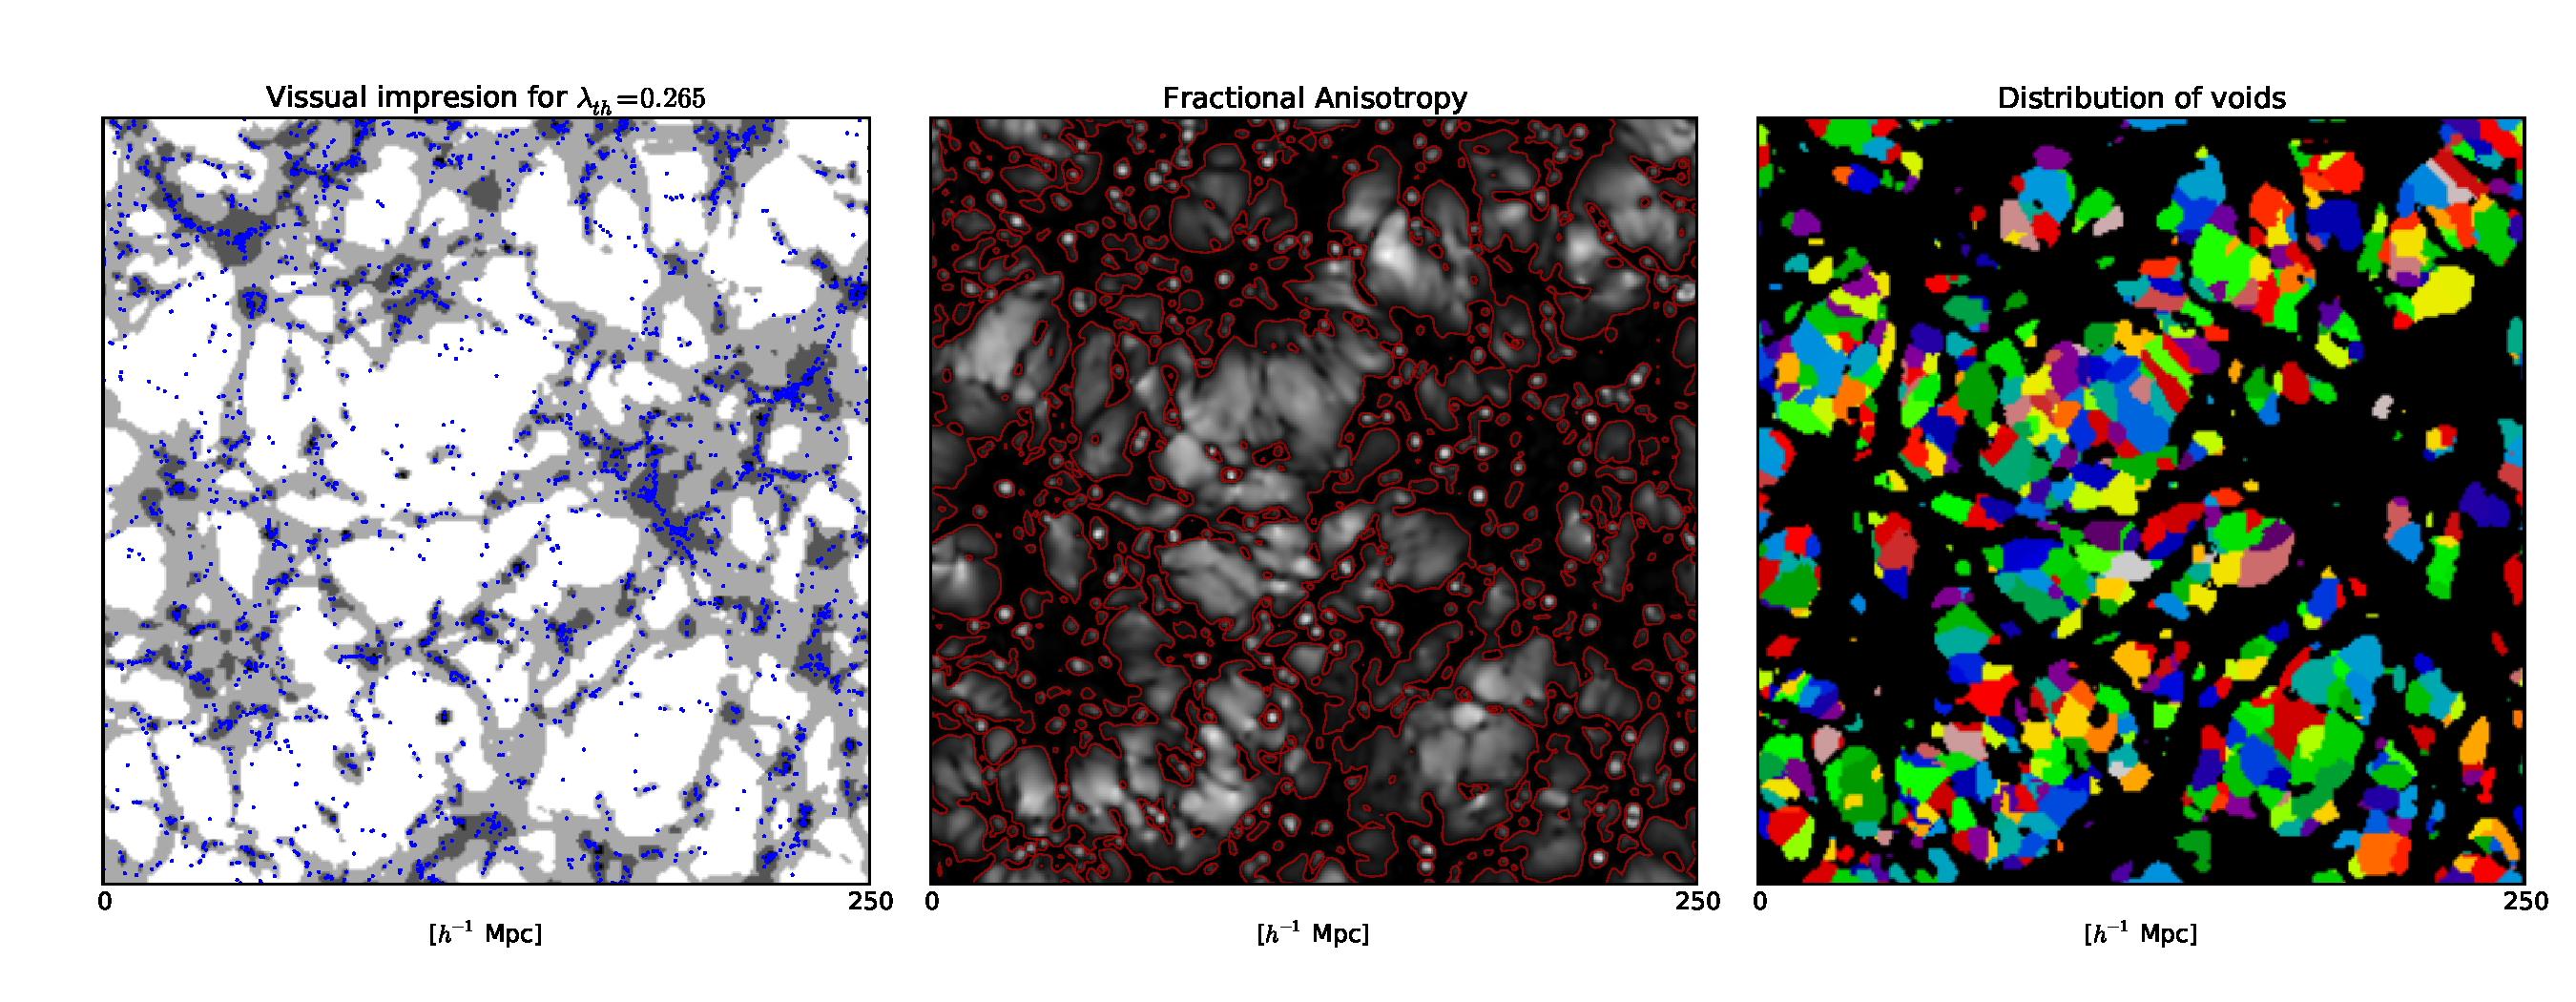
\includegraphics[trim = 16mm 10mm 5mm 12mm, clip, keepaspectratio=true,
  width=0.73\textheight]{./figures/cosmicweb_FA_Tweb.pdf}
  \vspace{0.1 cm}
  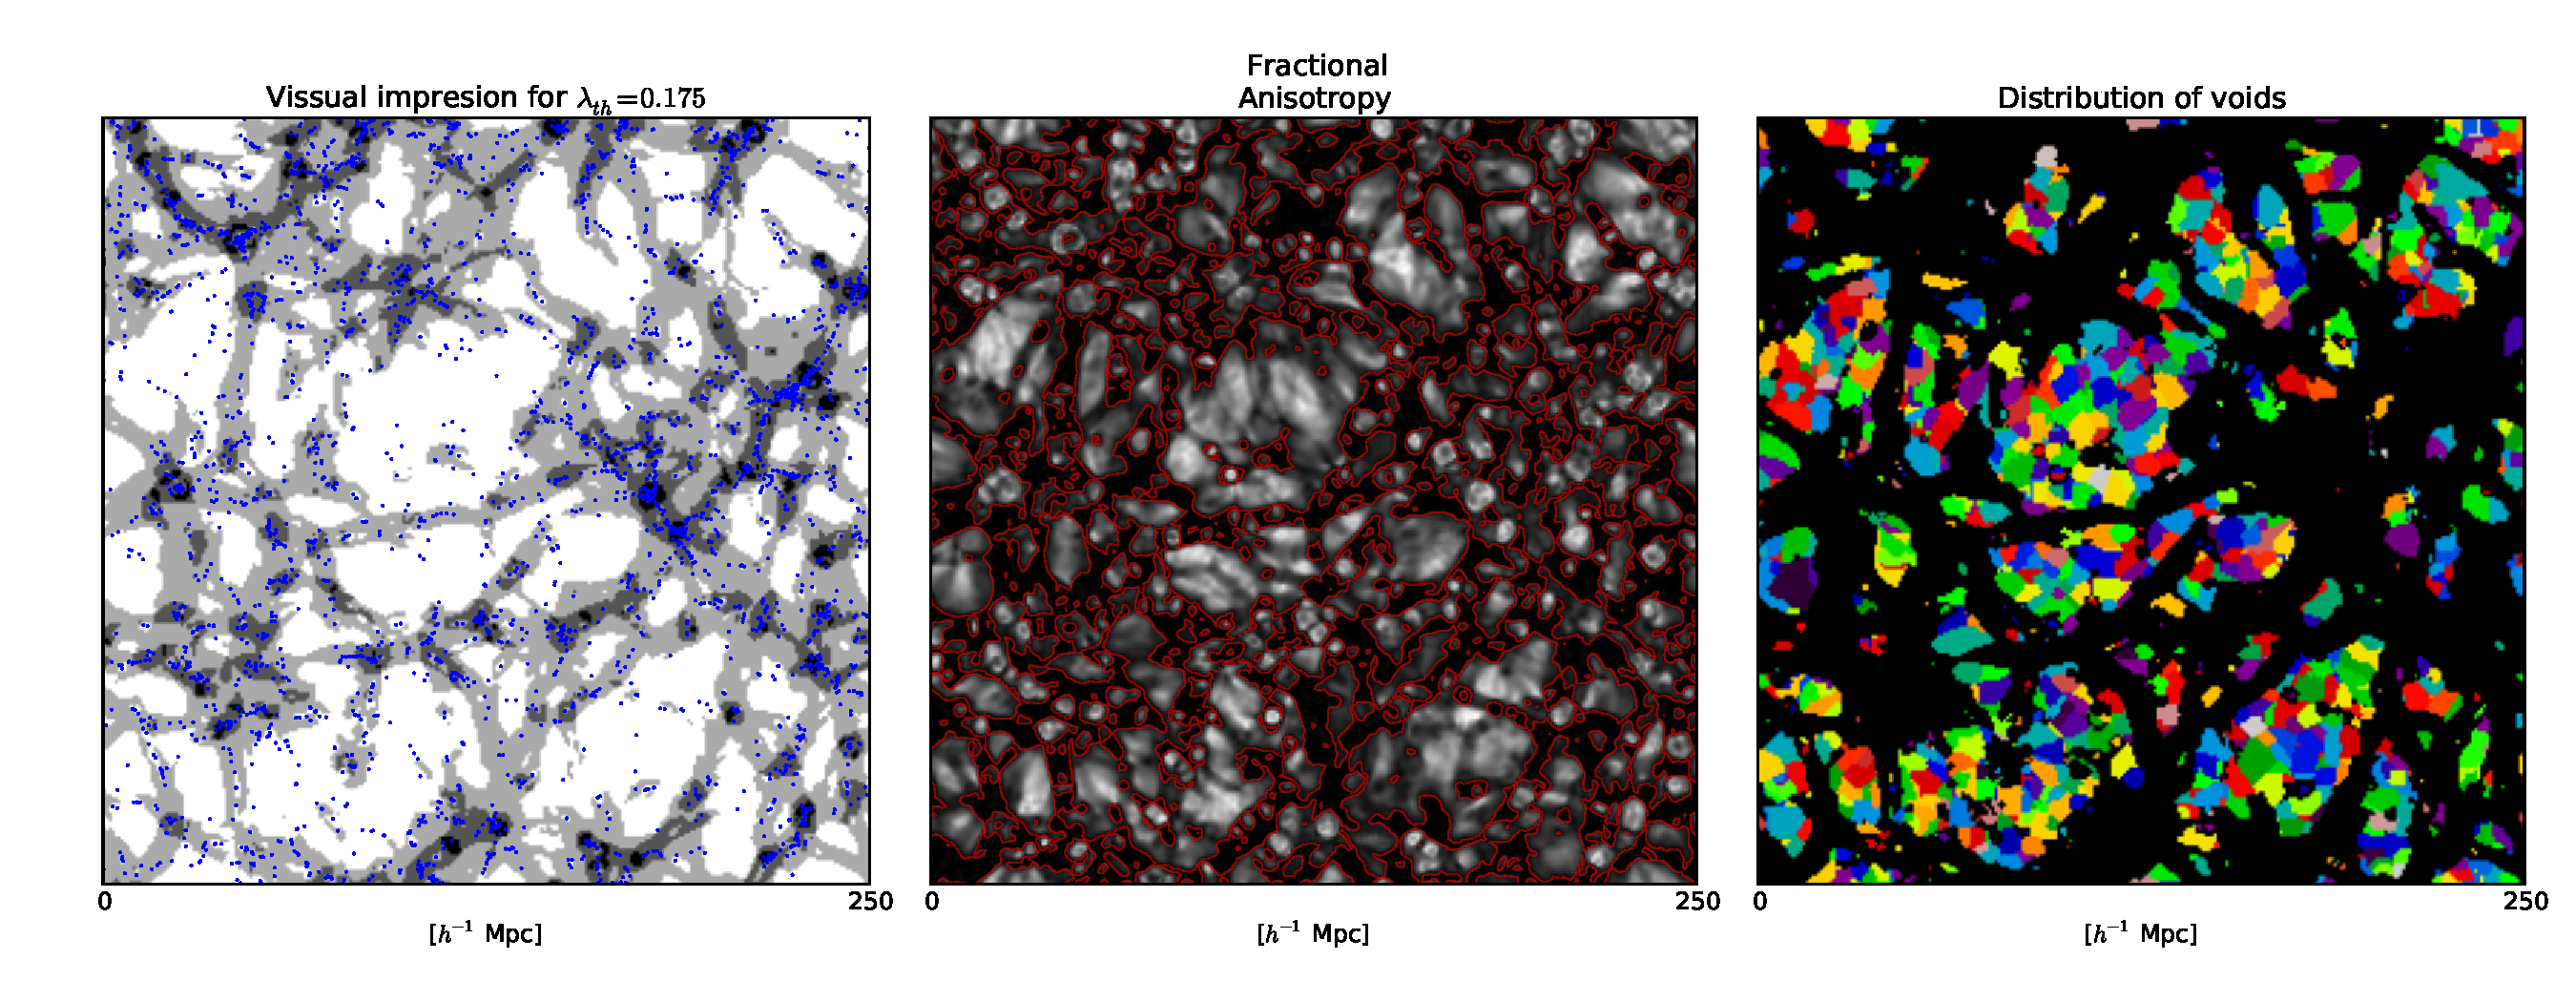
\includegraphics[trim = 16mm 10mm 5mm 12mm, clip, keepaspectratio=true,
  width=0.73\textheight]{./figures/cosmicweb_FA_Vweb.pdf}
  \vspace{0.1 cm}  
  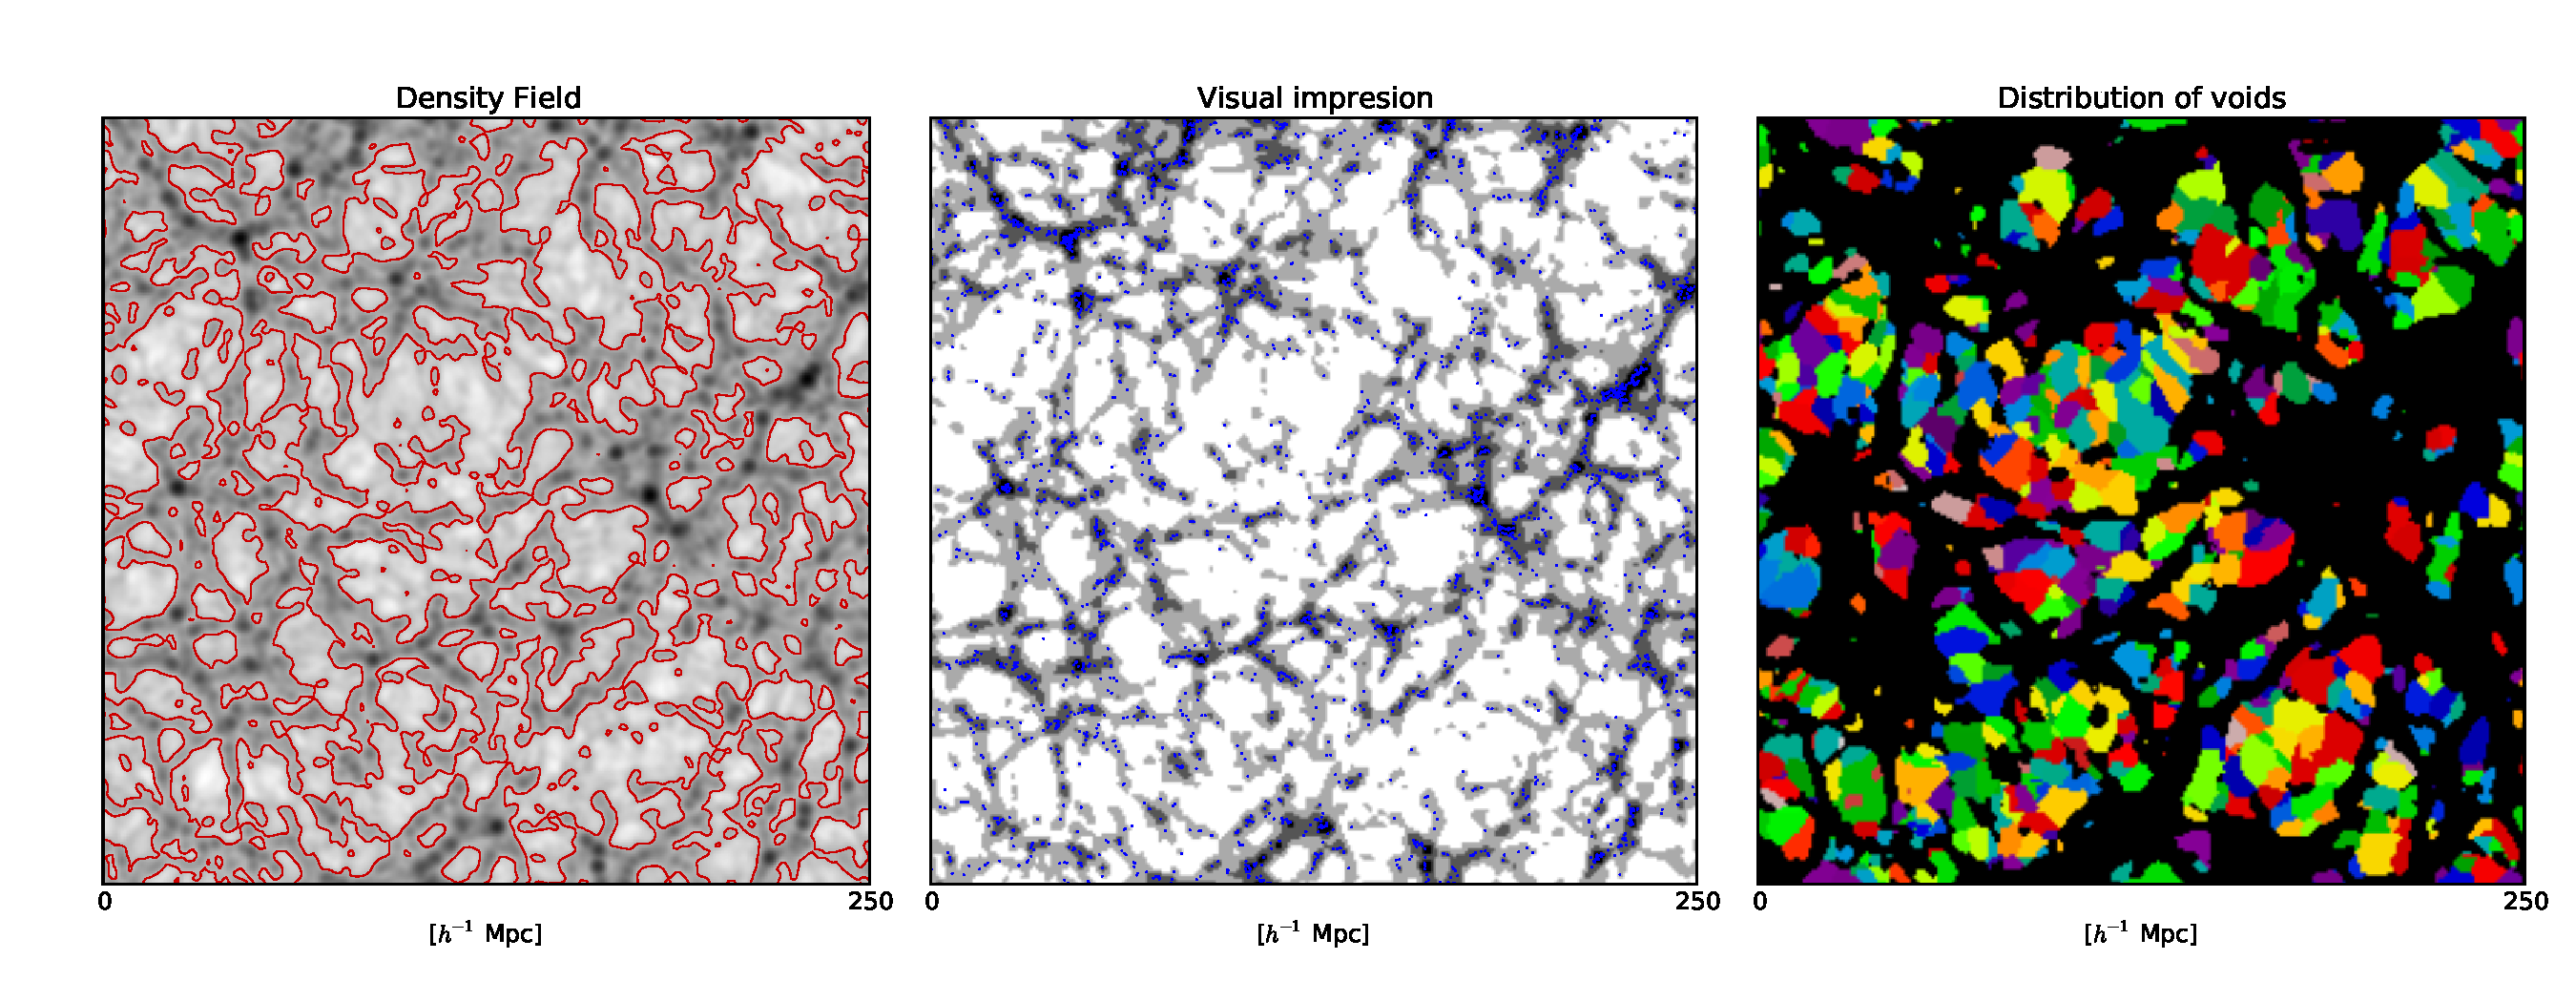
\includegraphics[trim = 16mm 10mm 5mm 12mm, clip, keepaspectratio=true,
  width=0.73\textheight]{./figures/cosmicweb_density.pdf}
  
  \captionof{figure}{\small Left panels show the visual impression of the 
  Cosmic Web for each web scheme (T-web, upper panels. V-web, middle 
  panels. Density, lower panels). It can be noticed each environment 
  sketched such that voids corresponds to white, sheets to gray, filaments 
  to dark gray and knots to black regions. Right panels show the fractional 
  anisotropy field for the same slide of the simulation and for each web 
  scheme. Black regions correspond to the maxim value, i.e. FA$=1$, while 
  white and light yellow regions to FA$=0$. It is worth noting the 
  degeneration of low values of FA for knots and central regions of voids, 
  thus indicating a high isotropy for both processes. In the same way, high 
  values of FA (FA $\lesssim 1$) are consistent the anisotropic geometry 
  exhibited by filaments and very flat sheets.}

  \label{fig:FA_field}

  
\end{figure*}
%.........................................................................


%.........................................................................
%FIGURE 5: volume functions
\begin{flushleft}
\begin{figure*}
\centering

  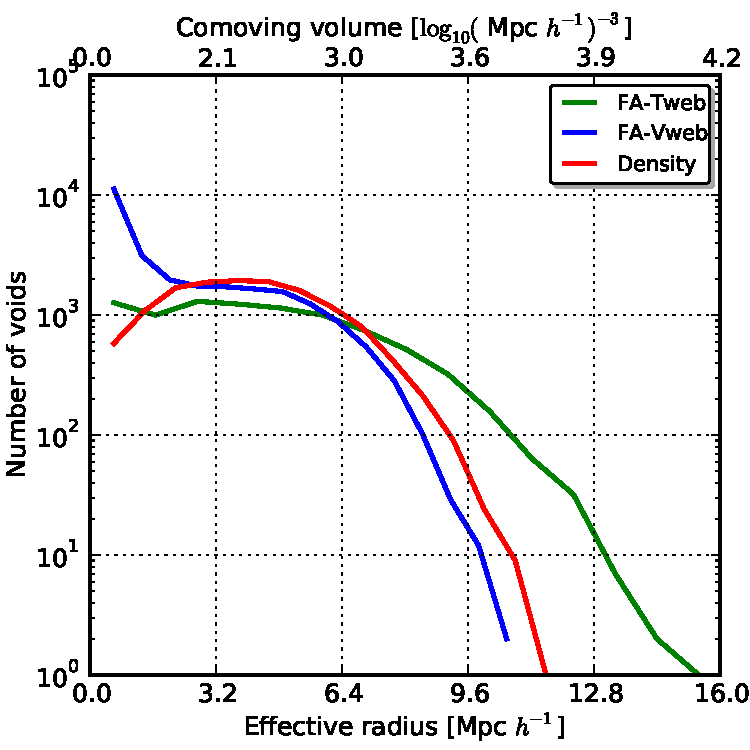
\includegraphics[trim = 0mm 0mm 0mm 0mm, clip, keepaspectratio=true,
  width=0.3\textheight]{./figures/voids_regions_volume_all.pdf}
  
  \captionof{figure}{\small Volume functions of voids catalogued by each 
  used scheme. Left panel (watershed transform over the FA field of the T-web 
  scheme). Central panel (over the FA field of the V-web scheme). Right panel 
  (over the density field). Gray curves correspond to voids without boundary 
  removal whereas black curves are associated to voids merged through boundary 
  removal process. Dotted lines correspond to original continuous fields, 
  while segmented lines correspond to fields with a 1st-order median filtering 
  and continuous lines to a 2nd-order median filtering.}

  \label{fig:volume_function}
  \vspace{0.1 cm}

\end{figure*}
\end{flushleft}
%.........................................................................


%.........................................................................
%FIGURE 6: Density profile of voids for each defined scheme
\begin{flushleft}
\begin{figure*}
\centering
  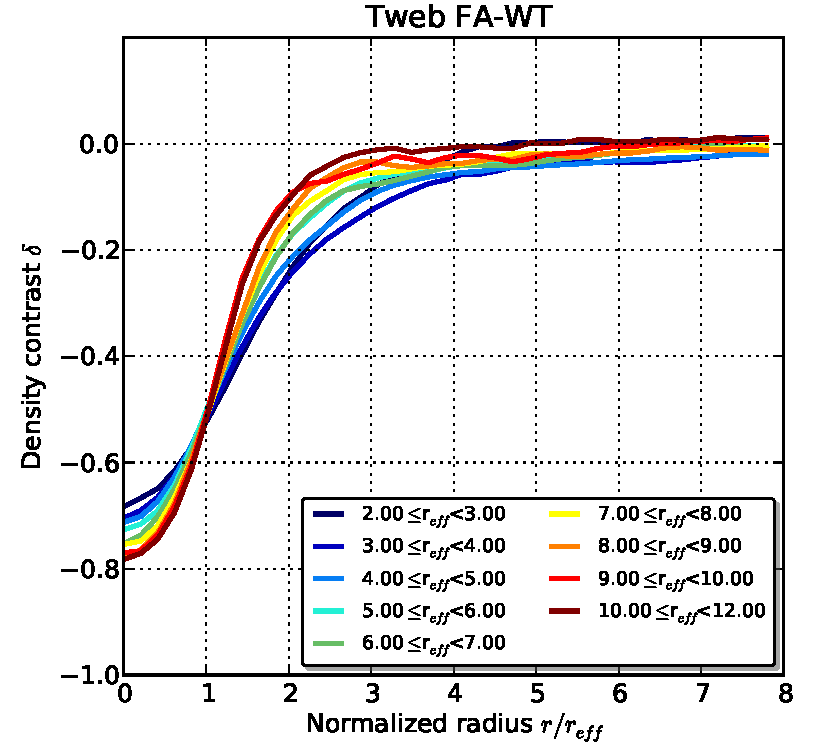
\includegraphics[trim = 1mm 2mm 4mm 0mm, clip, keepaspectratio=true,
  width=0.24\textheight]{./figures/voids_density_TwebFAG.pdf}
  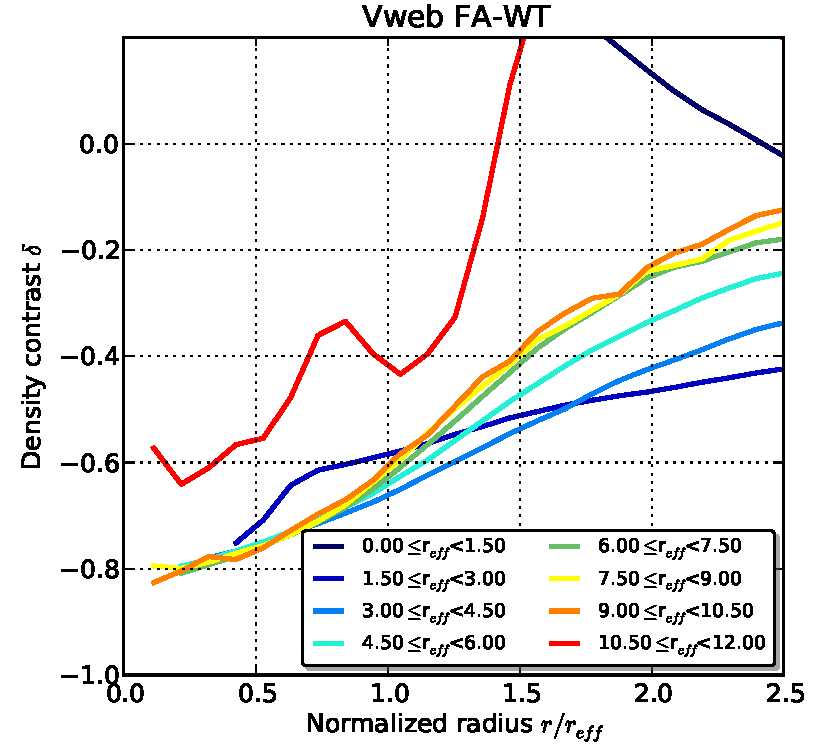
\includegraphics[trim = 1mm 2mm 4mm 0mm, clip, keepaspectratio=true,
  width=0.24\textheight]{./figures/voids_density_VwebFAG.pdf}
  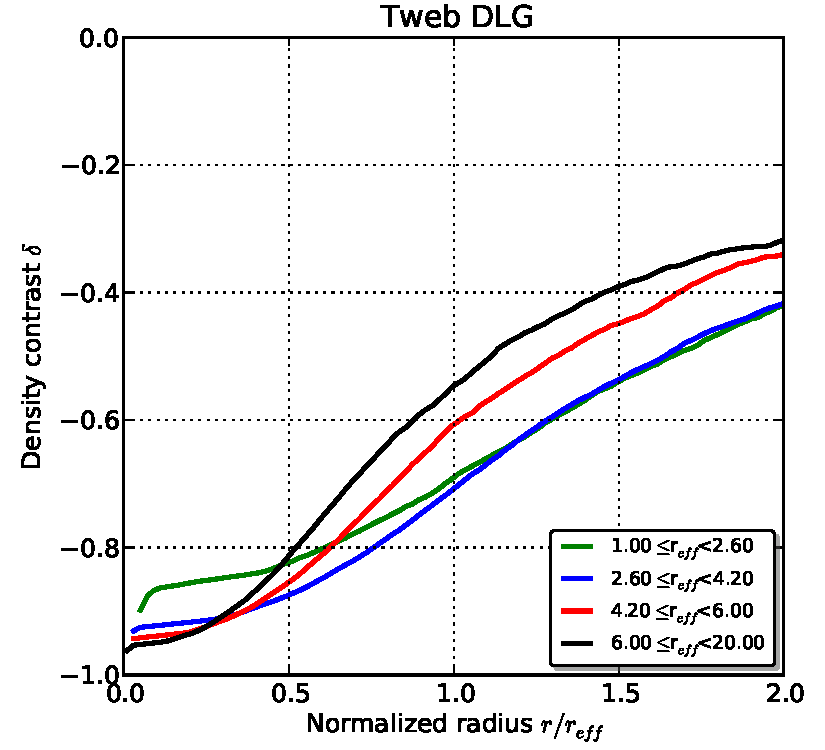
\includegraphics[trim = 1mm 2mm 4mm 0mm, clip, keepaspectratio=true,
  width=0.24\textheight]{./figures/voids_density_TwebDLG.pdf}
  
  \
  
  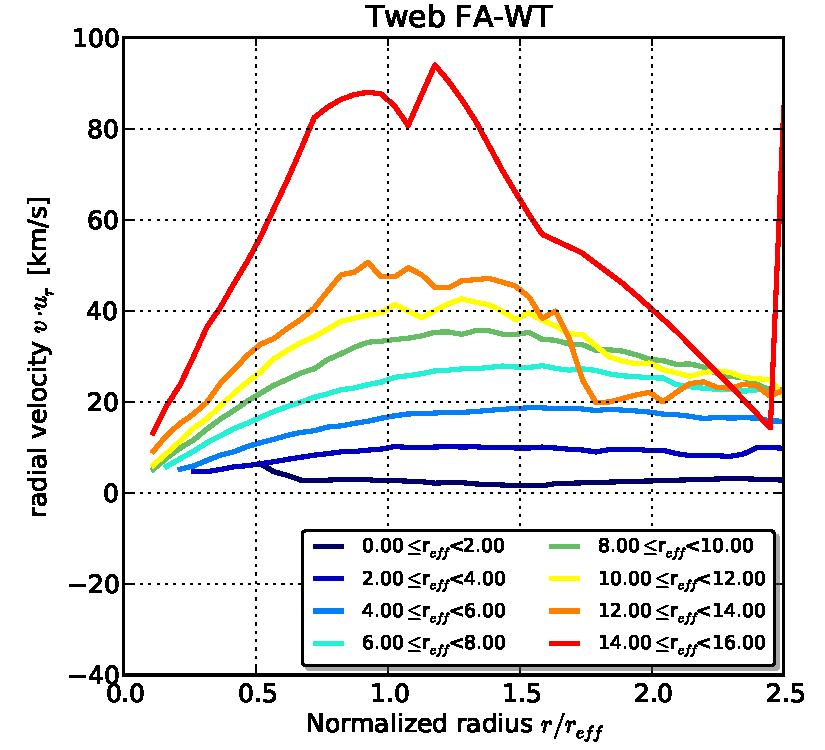
\includegraphics[trim = 1mm 2mm 4mm 0mm, clip, keepaspectratio=true,
  width=0.24\textheight]{./figures/voids_velocity_TwebFAG.pdf}
  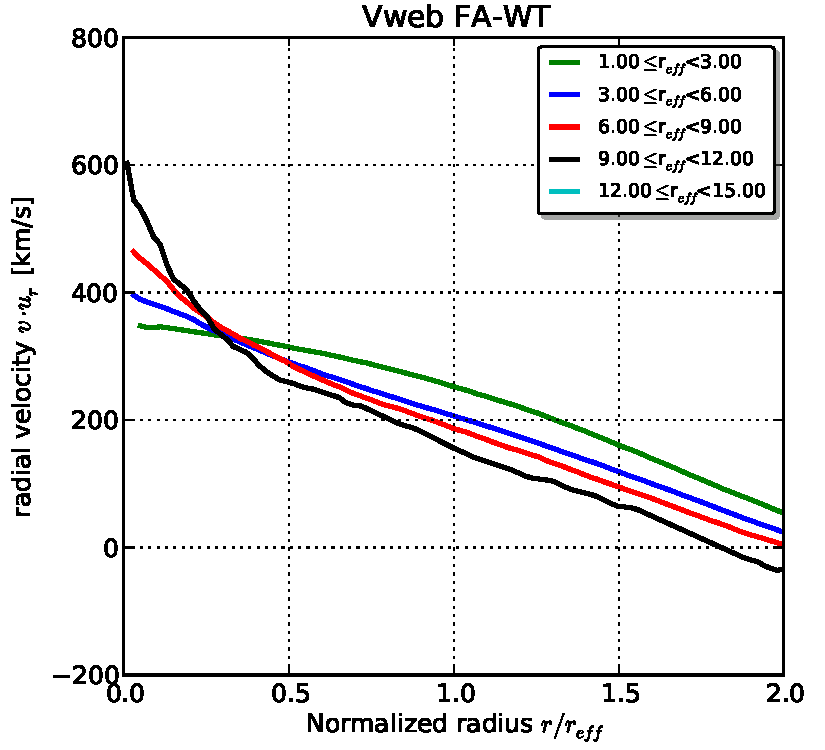
\includegraphics[trim = 1mm 2mm 4mm 0mm, clip, keepaspectratio=true,
  width=0.24\textheight]{./figures/voids_velocity_VwebFAG.pdf}
  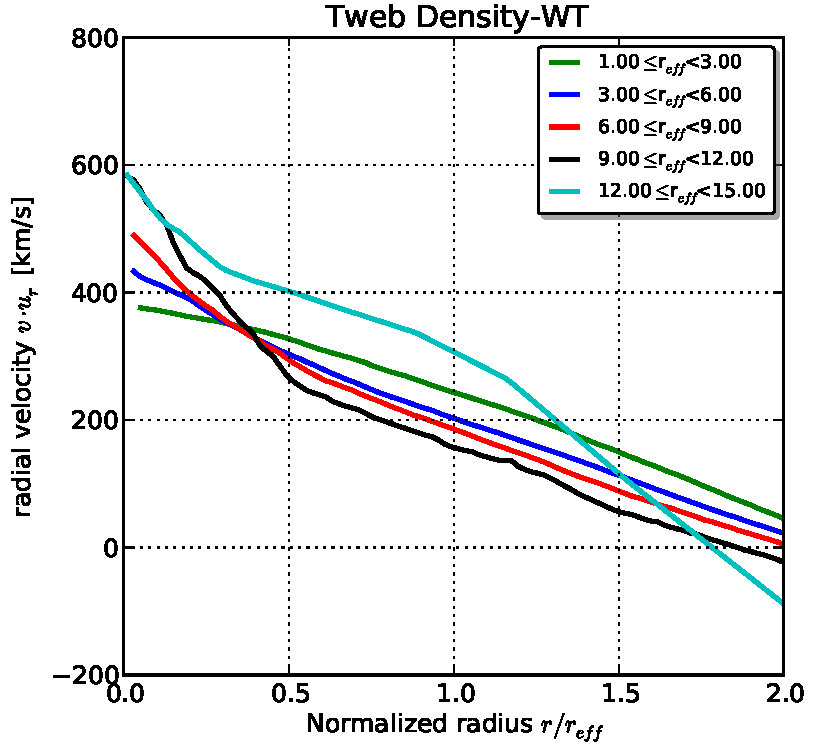
\includegraphics[trim = 1mm 2mm 4mm 0mm, clip, keepaspectratio=true,
  width=0.24\textheight]{./figures/voids_velocity_TwebDLG.pdf}
  
  \captionof{figure}{\small Density and velocity profiles of voids for 
  each finding scheme.}

  \label{fig:RhoVel}
  \vspace{0.1 cm}

\end{figure*}
\end{flushleft}
%.........................................................................


\end{document}
